\documentclass[titlepage=false,12pt]{scrreprt}

\usepackage[utf8]{inputenc}
\usepackage[T1]{fontenc}
\usepackage{lmodern}
\usepackage[ngerman]{babel}
\usepackage{amsmath}
\usepackage[backend=bibtex]{biblatex}
\usepackage{tikz}
\usepackage{amsthm}
\usepackage{amssymb}
\usepackage{xcolor}
\usepackage{framed}
\usepackage{tabto}
\usepackage{capt-of}
\usepackage{pgfplots} % loads tikz
\pgfplotsset{compat=1.7}
\usepackage{csquotes}
\usepgfplotslibrary{fillbetween}
\usetikzlibrary{intersections}
\usepackage{graphicx}
\graphicspath{{./../img/}}

\usepackage{listings}

\pgfdeclarelayer{bg}
\pgfsetlayers{bg,main}

\colorlet{shadecolor}{gray!15}

\usepackage{hyperref}
\hypersetup{
	colorlinks,
	citecolor=black,
	filecolor=black,
	linkcolor=black,
	urlcolor=black
}

\newtheorem{definition}{Definition}[chapter]
\AfterEndEnvironment{definition}{\noindent\ignorespaces}

\newcommand{\listingsettings}{%
	\lstset{%
		language=C++,			% Standardsprache des Quellcodes
		%numbers=left,			% Zeilennummern links
		%stepnumber=1,			% Jede Zeile nummerieren.
		%numbersep=5pt,			% 5pt Abstand zum Quellcode
		%numberstyle=\tiny,		% Zeichengrösse 'tiny' für die Nummern.
		breaklines=true,		% Zeilen umbrechen wenn notwendig.
		breakautoindent=true,	% Nach dem Zeilenumbruch Zeile einrücken.
		postbreak=\space,		% Bei Leerzeichen umbrechen.
		tabsize=2,				% Tabulatorgrösse 2
		basicstyle=\ttfamily\footnotesize, % Nichtproportionale Schrift, klein für den Quellcode
		showspaces=false,		% Leerzeichen nicht anzeigen.
		showstringspaces=false,	% Leerzeichen auch in Strings ('') nicht anzeigen.
		extendedchars=true,		% Alle Zeichen vom Latin1 Zeichensatz anzeigen.
		captionpos=b,			% sets the caption-position to bottom
		%backgroundcolor=\color{ListingBackground}, % Hintergrundfarbe des Quellcodes setzen.
		xleftmargin=0pt,		% Rand links
		xrightmargin=0pt,		% Rand rechts
		frame=single,			% Rahmen an
		frameround=ffff,
		rulecolor=\color{darkgray},	% Rahmenfarbe
		%fillcolor=\color{ListingBackground},
		keywordstyle=\color[rgb]{0.133,0.133,0.6},
		commentstyle=\color[rgb]{0.133,0.545,0.133},
		stringstyle=\color[rgb]{0.627,0.126,0.941},
		aboveskip=1.5em,
	}
}

\clubpenalty = 10000 % schließt Schusterjungen aus (Seitenumbruch nach der ersten Zeile eines neuen Absatzes)
\widowpenalty = 10000 % schließt Hurenkinder aus (die letzte Zeile eines Absatzes steht auf einer neuen Seite)
\displaywidowpenalty=10000

\bibliography{bibliography}

\title{MVVM: Model-View-ViewModel}
\subtitle{Advanced Softwareengineering - DHBW Stuttgart}
\author{Nico Vogel, Lukas Sopora}
\date{31.01.2020}

\begin{document}
\maketitle
	
{\renewcommand\clearpage\relax
	\tableofcontents}
\newpage

\chapter{Einleitung zu MVVM}

\section{Anwendungsbereiche von MVVM}

Bereits vor der Veröffentlichung von MVVM wurden bei der Entwicklung von Applikationen mit einer grafischen Benutzeroberfläche Design Patterns angewandt, 
mit denen der Programmcode sinnvoll in Komponenten eingeteilt werden konnte, mit dem Ziel, den Überblick und die Wartbarkeit der Applikation für den Entwickler zu vereinfachen.
\\\\
\noindent
Das bekannteste dieser Patterns, welches auch heute noch häufige Verwendung findet, ist das Model-View-Controller (MVC) Pattern.
Aus diesem entwickelte sich auch das Model-View-Presenter (MVP) Pattern, woraus 2004 wiederum das Presentation-Model (PM) hervorging.
2005 wurde schließlich vom Microsoft Architekten John Gossmann das Model-View-ViewModel (MVVM) Pattern als Spezialisierung des Presentation Model vorgestellt.
Seitdem wird es vor allem in C\# im Zusammenhang mit WPF, aber auch in Delphi, Silverlight und AngularJS angewandt.
\\\\
\noindent
Alle oben erwähnten Patterns verfolgen denselben Ansatz, den Programmcode sinnvoll aufzuteilen und die Oberflächenbeschreibung der Benutzeroberfläche von der Programmlogik zu trennen. \par

\section{Was ist das Problem das MVVM angeht?}

Das MVVM Pattern nimmt in erster Linie eine ordnungsgemäße Trennung von Geschäfts- und Präsentationslogik vor und
behebt somit das Problem der starken Kopplung von User Interface Komponenten und der eigentlichen Programmlogik.
Dieser Ansatz bringt einige Vorteile mit sich und erleichtert die Arbeit der Entwickler im Vergleich zu klassischen
Herangehensweisen.\\
\\
Die Wartbarkeit der Applikation verbessert sich erheblich, da sich Entwickler auf die Wartung einzelner kleinerer
Komponenten konzentrieren können und nicht das gesamte System im Blick behalten müssen. Auch die Wiederverwendbarkeit
von Code steigt durch die Möglichkeit der Abstraktion des User Interfaces. Dadurch erhöht sich auch die Skalierbarkeit.\\
\\
Ein weiterer Vorteil ist, dass sich solche eigenständigen Komponenten besser und automatisiert testen lassen können.
Spezifische Test Cases lassen sich so mit Unit Tests gut umsetzen.
\\
Außerdem können sich Backend Entwickler auf die Programmlogik konzentrieren, währen Frontend Entwickler den Fokus
auf die Benutzeroberfläche und das Design legen können. Voraussetzung dafür sind klare Definitionen von
Anforderungen und Schnittstellen vor und Beginn der Entwicklung.\\
\\
Frameworks, wie MVVMCross ermöglichen die Anwendung von MVVM auf beispielweise mobile Cross-Platform Anwendungen.

\chapter{Wie ist MVVM aufgebaut?}

MVVM besteht aus mehreren Komponenten, die ineinandergreifen. Die drei 
größten sind Model, View und ViewModel. Dabei wird das Zusammenspiel 
der Komponenten in der Abbildung 2.1 dargestellt. Während das ViewModel das Model
nur aufruft, beziehungsweise es verwendet, kommunizieren View und ViewModel über
Bindings bidirektional. Dabei ist allerdings zu erwähnen, dass die View das ViewModel
kennt, aber nicht anders herum. Das ViewModel stellt lediglich Daten und Funktionalitäten
zur Verfügung, weiß aber nicht, wo und wie diese außerhalb der Klasse verwendet werden.

\begin{figure}[h]
	
\includegraphics[width=\textwidth]{MVVM.png}
	\caption[]{DataBinding}
\end{figure}

\section{Komponenten}

\paragraph{Model}

Das Model umfasst nur Daten und maximal noch Logik für die Daten. 
Im C\# Umfeld spricht man auch von POCO (Plain old Control Object) 
oder in Java POJO (Plain old Java Object).
\\
Das folgende Beispiel beschreibt eine Schülerklasse die der Definition 
eines Models entspricht.

\lstinputlisting{./../code/student.cs}

\paragraph{ViewModel}

Mithilfe des ViewModels werden Informationen und Funktionen zusammengefasst
in eine Klasse, damit eine View diese verwenden kann. Das ViewModel verwenden zur 
Informationsbereitstellung die Models. Die bereitgestellten Funktionen sind
entweder in dem ViewModel selbst oder in separaten Klassen implementiert.

\paragraph{View}

Die View ist ausschließlich zur Darstellung der Inhalte und Bereitstellen der
Funktionen über Schaltflächen oder Ähnliches gedacht. Dabei wird in der View
Binding verwendet, um Inhalte und Funktionen von dem ViewModel zu verwenden.
In der Regel wird jeder Instaz einer View genau eine ViewModel Instanz als DataContext
Eigenschaft zugewiesen.

\section{Kommunikation}

Nachdem nun die Hauptkomponenten beschrieben sind, fehlt noch wie diese miteinander 
kommunizieren. Hierbei werden Model Instanzen zwischen der View und dem ViewModel ausgetauscht.
Dieser Austausch und der Aufruf von Funktionalitäten des ViewModels werden über Binding, 
Events und Commands realisiert.

\paragraph{Binding}

Binding gibt es grundsätzlich in zwei Variationen. Diese sind in Abbildung 2.1 dargestellt. \textbf{OneWay Binding}
lässt Kommunikation nur in eine Richtung zu, somit von dem ViewModel zur View und umgekehrt.
Letzteres nennt man in C\# auch \textbf{OneWayToSource}. Die zweite Variante ist \textbf{TwoWay Binding} ermöglicht
der View als auch dem ViewModel Informationen an den jeweils anderen zu senden. Zusätzlich ist 
bei WPF das \textbf{OneTime Binding} vertreten, wobei die Zieleigenschaft nur beim Start der Applikation 
oder, wenn sich die DataContext Eigenschaft ändert, also wenn der View Komponente ein neues 
ViewModel zugewiesen wird.

\begin{figure}[h]
	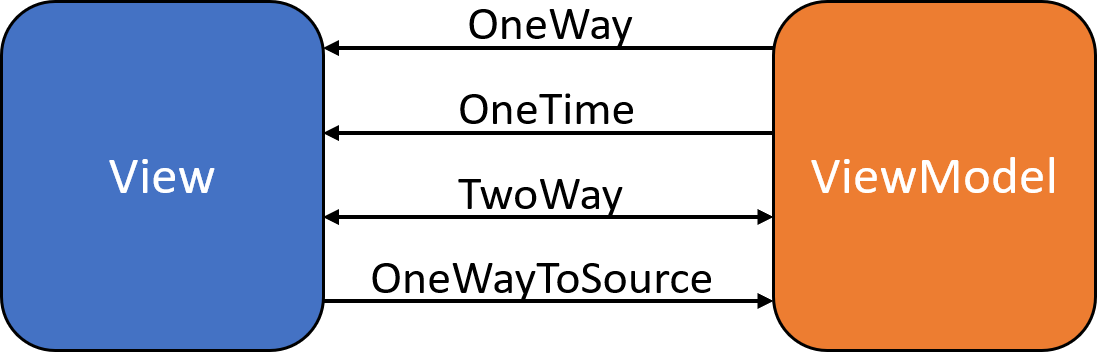
\includegraphics[width=\textwidth]{Wpf_Binding.png}
	\caption[]{DataBinding}
\end{figure}


\paragraph{Event}

Events sind Ereignisse von UI Komponenten, auf welche sich andere Komponenten registrieren 
können, um so zusätzlichen Code auszuführen. Es gibt eine breite Menge an Events die
von Komponenten zur Verfügung gestellt wird. Beispiele für Events können Hover-Ereignisse
oder ein Doppelklick auf eine Komponente sein.
Diese können standardmäßig nicht and das ViewModel
gebunden werden, sondern rufen eine Funktion in der Code-Behind Datei auf.
Soll ein Event eine Funktionalität im ViewModel aufrufen, kann dafür in C\# eine Verlinkung in der
Code-Behind Datei erstellt werden. Durch die Verwendung von zusätzlichen Bibliotheken, wie
Blend Interactivity Features, können Events über Umwege an Commands gebunden werden.

\paragraph{Command}

Commands sind Events, die über Binding verwendet werden können. Hierbei ist eine schlechte
Abdeckung gegeben, weshalb häufig auf Events zurückgegriffen werden muss. Ein Command
beinhält auch keine Informationen, sondern ist nur ein Trigger einer Methode. Ein Beispiel
ist Button klick.

\section{Wo ordnet sich MVVM in Application Layer ein?}

Da in Anwendung in der Regel auch mit Strukturpattern realisiert wird, wird in der Abbildung X
das MVVM Pattern in das Application Layer Model eingefügt. Hierbei ist wichtig, dass das
ViewModel sowohl in der Presentation, als auch in der Business Layer vertreten ist. Das kommt
daher, dass das ViewModel einerseits Methoden und Properties für die View aggregiert und andererseits
Business Code ausführt.  

ABBILDUNG X - Application layered

\chapter{Beispiel mit C\# und WPF}

Das MVVM Pattern findet vor allem in WPF (Windows Presentation Foundation) Applikationen, die in C\#
implementiert sind, Anwendung.
Zur Veranschaulichung wurde ein Prototyp für ein Schulverwaltungssystem implementiert, welcher
grundlegende Funktionalitäten enthält, die zur Veranschaulichung des MVVM Patterns dienen.\\
Neben den Grundlagen der Verwendung des Patterns werden auch Vor- und Nachteile anhand von konkreten
Beispielen, die bei der Implementierung aufgetreten sind, vorgeführt.

\section{Model}

Im System sollen Schüler und Lehrer repräsentiert werden. Demnach wurden zwei entsprechende
Klassen für diese Entitäten implementiert. Zusätzlich wurde eine Superklasse Person hinzugefügt.

\begin{figure}[h]
	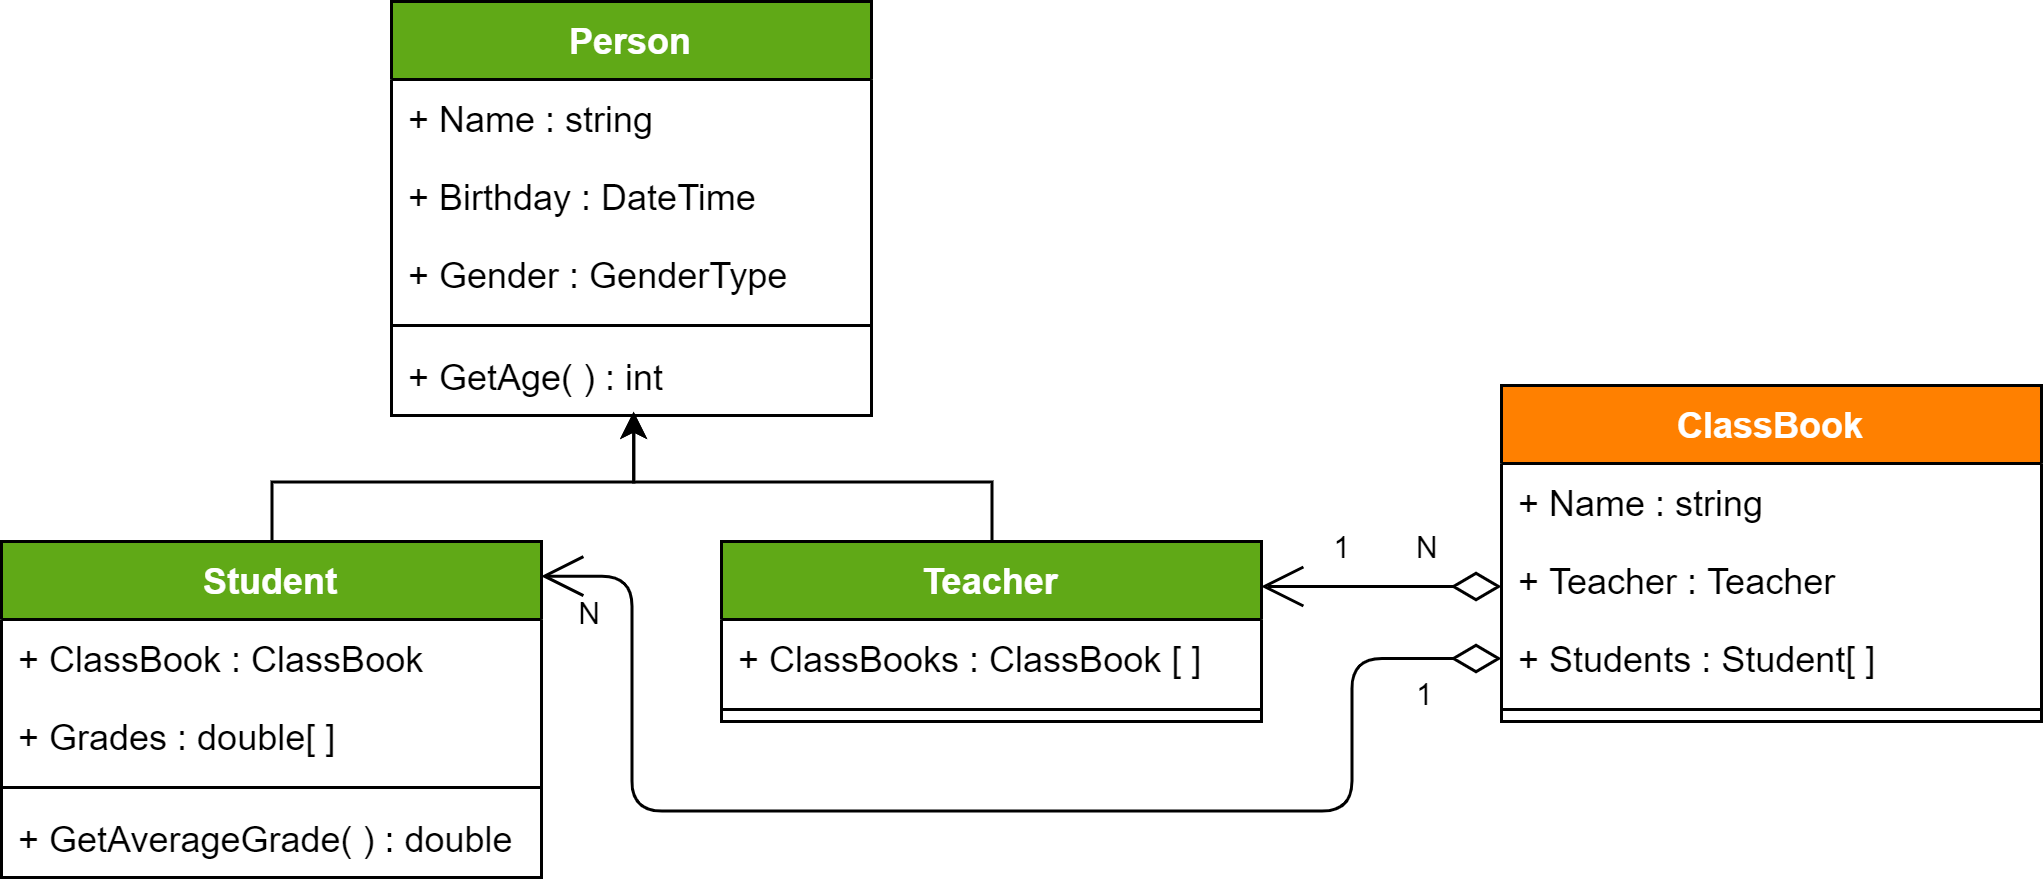
\includegraphics[width=\textwidth]{SchoolPersonUML.png}
	\caption[]{Personen Model}
\end{figure}

\noindent
Ein Schüler ist genau einer Klasse zugewiesen, während ein Lehrer auch für mehrere Klassen verantwortlich
sein kann. Anders herum hat eine Klasse genau einen Lehrer und eine beliebige Anzahl an Schülern.
Durch die bidirektionale Referenz zwischen Personen und Klassen kann beispielweise von einem Schüler
auf seine Klasse zugegriffen werden und von dort wiederum auf den Schüler. Dabei existiert zur Laufzeit von einer
spezifischen Person oder Klasse immer nur eine Instanz.

\chapter{Vergleich zwischen MVVM und MVC}

In diesem Abschnitt wird beschrieben wie sich MVVM zu MCV (Model View Controller) unterscheidet. 
Zu Beginn wird das MVC Pattern erläutert, um daraufhin die Unterschiede hervorzuheben. 

\paragraph{Was ist MVC?}

Das Model View Controller Pattern ist erstmals im Kontext der Programmiersprache SMART verwendet 
worden. In diesem Fall sind Komponenten, wie Eingabefelder, mit dem MVC Pattern realisiert worden.
Mit dem Aufkommen von komplexeren Sprachen ist auch der Scope von MVC gewachsen. Bei TODO(passende Sprache/Framework einsetzen)
entspricht die View einer Komponente oder Seite.

Jede der drei Bestandteile von MVC hat seine eigene Aufgabe. Das Verhältnis unter den Komponenten
ist in Abbildung X dargestellt. Die View ist für die Darstellung und
Animation zuständig. Das Model stellt die Daten zur Verfügung, die in der View dargestellt werden.
Der Controller verbindet View und Model, da diese sich nicht kennen. Somit steht der Controller 
über der View und dem Model, wodurch Model und View entkoppelt sind, aber dafür eine starke Bindung
zum Controller besteht. 

ABBILDUNG X - MVC

\paragraph{Vergleich der beiden Pattern}

Während bei dem MVC Pattern der Controller das Verbinden der Komponenten übernimmt, wird das
in dem MVVM Pattern über Binding realisiert und ein externes System löst das Binding am Ende auf.
Bei MVC kennt die View das Model nicht, aber bei MVVM ist der View das ViewModel bekannt.
Das wird auch in der Abbildung X dargestellt durch die Verbindungen der Komponenten.

TODO vielleicht noch bissel mehr dazu sagen

ABBILDUNG X - MVC vs MVVM

\chapter{Kritische Betrachtung des MVVM Patterns}



Pro

<span class="text-left">

- flexibel
- steile Lernkurve (OOP, Testing, Binding)
- gut testbar

</span>
</div>

<div class="rdiv">

Con

<span class="text-left">

- viel code für wenig resultat
- XAML Notation umfangreich
- Binding undurchsichtig

</span>

\end{document}